% !TeX root = ../index.tex
\documentclass[../index.tex]{subfiles}

\begin{document}
    \section{Wykład}
        W zależności od masy ewolucja gwiazdy może przebiegać w bardzo zróżnicowany sposób. Skutkuje to różnym czasem trwania procesu i różnymi charakterystykami obiektów, na których ten proces się kończy. Do śledzenia przebiegu ewolucji gwiazdy stosuje się kilka alternatywnych sposobów:
        \begin{enumerate}
            \item \textbf{Diagram \(\log \rho_c\) – \(\log T_c\)} – obrazuje zmianę warunków panujących we wnętrzu gwiazdy pod wpływem zmiany składu chemicznego.
            \item \textbf{Diagram H-R} – ilustruje zmiany gwiazdy, które można weryfikować bezpośrednią obserwacją.
            \item \textbf{Diagram Kippenhahna} – przedstawia zmiany w całej strukturze gwiazdy w funkcji czasu.
        \end{enumerate}
        Poniżej widać diagram \(\log \rho_c\) – \(\log T_c\) z wyróżnionymi czterema obszarami, na których w jądrze panują inne równania stanu (od lewej: ciśnienie zależy od promieniowania, gaz doskonały, gaz fermiego nierelatywistyczny, gaz fermiego relatywistyczny):
        \begin{center}
            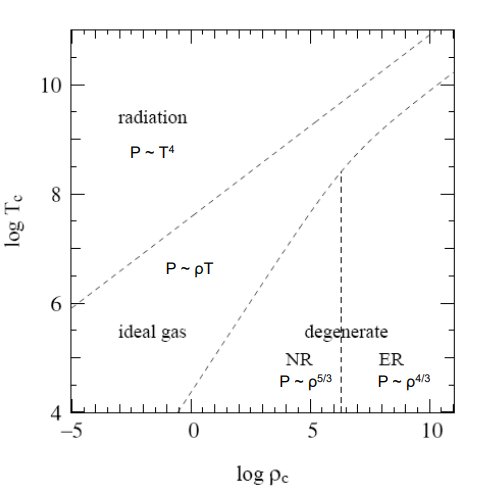
\includegraphics[width=12cm]{images/pustyLogRho_CT_C.png}
        \end{center}
        \subsection{Ewolucja gwiazd średnio masywnych}
            Poniżej widać ścieżki ewolucyjne gwiazd o masach 15, 7, 2 i 1 mas Słońca:
            \begin{center}
                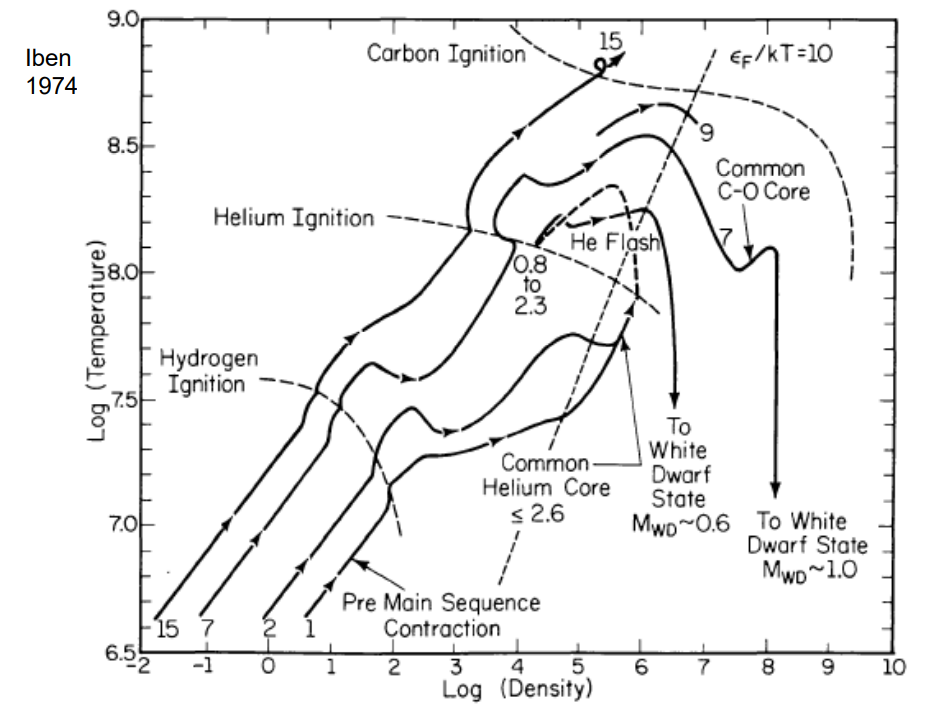
\includegraphics[width=12cm]{images/logRho_CT_C.png}
            \end{center}
            Jak widać najcięższa gwiazda w żadnym momencie nie opuszcza strefy gazu doskonałego i tylko one przekraczają linię oznaczającą zapłon węgla. Pozostałe ostatecznie skręcają w kierunku obszaru gazu zdegenerowanego, gdzie kończą jako białe karły. Gwiazdy o masach 0.8 – 2.3 mas Słońca inicjują zapłon helu w warunkach degeneracji. Dochodzi wówczas do \textbf{błysku helowego}(więcej o nim później). Gwiazdy o mniejszej masie nie zapalają helu wcale.\\
            Ilustracja poniżej pokazuje wędrówkę gwiazd po wykresie H-R w wyniku ich ewolucji:
            \begin{center}
                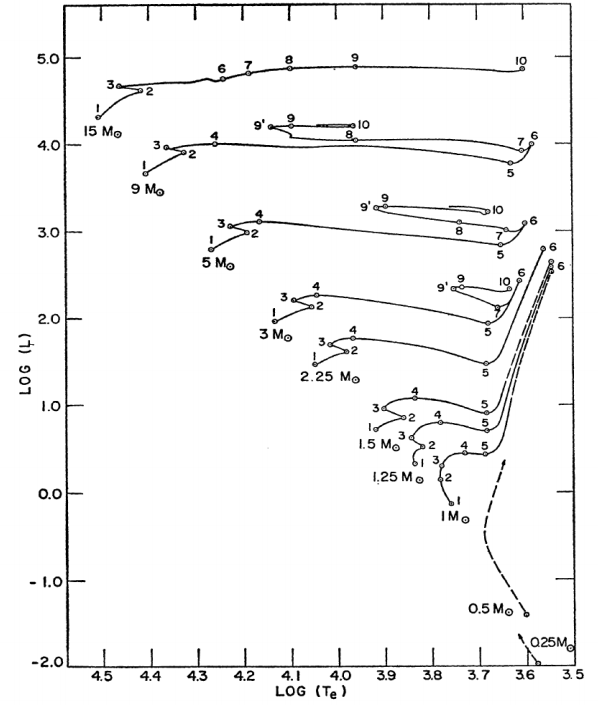
\includegraphics[width=10cm]{images/ewolucjaGwiazdHRII.png}
            \end{center}
            Liczby przy różnych krzywych odpowiadają tym samym etapom ewolucji (ale niekoniecznie temu samemu czasowi – ewolucje przebiegają w różnym tempie). Jak widać, mimo kurczenia się jądra (w celu syntezy ciężkich pierwiastków niż wodór) całkowity rozmiar gwiazdy zwiększa się (gwiazdy stają się \textbf{czerwonymi olbrzymami}). Otoczka reaguje lustrzanie do jądra – jeśli jądro się kurczy to otoczka się rozrasta i vice versa. Efekt ten spowodowany jest zmianami w energii grawitacyjnej jądra. Poniżej na wykresie Kippenhahna widać zobrazowanie tego procesu:
            \begin{center}
                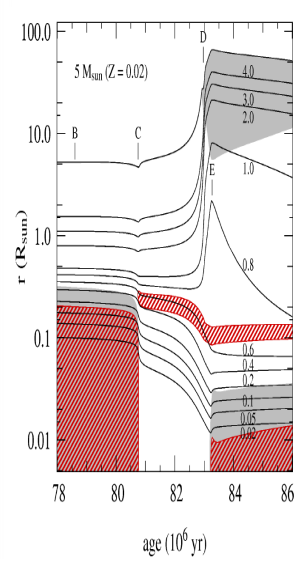
\includegraphics[width=6cm]{images/ewolucjaGwiazdKippenhahn.png}
            \end{center}
            Czerwony obszary to te, w których zachodzą reakcje jądrowe, a szare to obszary konwekcji.\\
            Do \textbf{błysku helowego} dochodzi, gdy podczas przechodzenia na spalanie helu, jądro gwiazdy jest w stanie zdegenerowanym. W przypadku degeneracji ciśnienie nie zależy od temperatury – nie działa mechanizm regulujący tempo reakcji(reakcja \(3\alpha\)). Wydzielana energia zwiększa temperaturę, co przyspiesza tempu zachodzenia tego procesu. Odpowiednio duży wzrost temperatury przy stałym ciśnieniu wywołuje zniesienie degeneracji i przejście gwiazdy w stan gazu doskonałego. W momencie błysku wydzielona jest energia 10 miliardów słońce, ale sama gwiazda przygasa, ponieważ większość tej energii konsumowana jest na likwidacje degeneracji i zwiększanie rozmiarów jądra (regulacja tempa procesu).\\
            Po przejściu na spalanie helu gwiazdy zajmują miejsce na \textbf{gałęzi horyzontalnej} wykresu H-R poruszając się w lewo, a po pewnym czasie skręcają w prawo i do góry – na tzw. \textbf{asymptotyczną gałąź olbrzymów}. W obrębie tych procesów budowa gwiazdy znacznie się zmienia:
            \begin{center}
                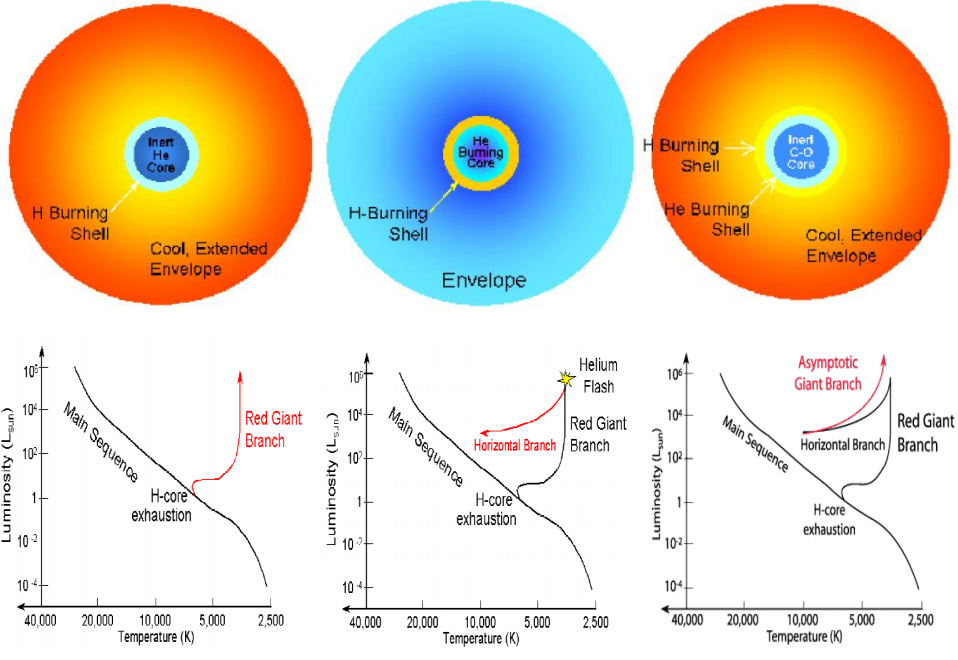
\includegraphics[width=14cm]{images/ewolucjaGwiazdOlbrzymy.png}
            \end{center}
            Na asymptotycznej gałęzi olbrzymów można wyróżnić jadro węglowo-tlenowe powłokę, w której spalany jest hel i powłokę, w której spalany jest wodór oraz otoczkę (nawet po ustaniu procesu spalania helu czy wodoru w jądrze powstają wokół niego otoczki, w których te procesy nadal zachodzą, jednocześnie będąc źródłem paliwa dla niższych warstw). W zasadzie można wyróżnić dwa różne byty – malutkie (ok 4 x promień Ziemi) jądro i bardzo rozrzedzona chmura wodoru zajmującą kulę o promieniu kilkuset większym niż Słońce.\\
            Tempo zachodzenia reakcji w obu powłokach podlega powtarzającym się zmianom. Krótkotrwałym wzrostom towarzyszy gwałtowne rozprężanie, które ogranicza tempo, po czym stopniowa kontrakcja powoduje jego zwiększenie do poziomu skutkującego kolejnym rozprężaniem warstwy. To zjawisko nazywa się \textbf{pulsami termicznymi}:
            \begin{center}
                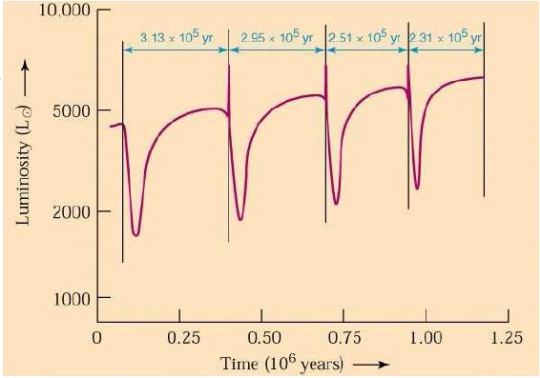
\includegraphics[width=12cm]{images/pulsyTermiczne.png}
            \end{center}
            Zaburzenia przenoszą się do otoczki, gdzie ich amplituda ulega zwiększeniu. Skutkuje to powtarzającym się odrzucaniem zewnętrznych fragmentów otoczki – powstają \textbf{mgławice planetarne}. W rezultacie przez pewien okres gwiazda staje się wielkim obłokiem rzadkiej materii z małej wielkości świecącym i gęstym jądrem wewnątrz. Po tysiącach lat obłok rozwiewa się zupełnie i jedyne co pozostaje to owo jądra – gwiazda staje się \textbf{białym karłem}.
        \subsection{Ewolucja gwiazd masywnych}
            W przypadku gwiazd o dużej masie, jądra nie ulegają degeneracji oraz są w stanie syntezowa pierwiastki cięższe niż hel. Istotnym aspektem ewolucji tych gwiazd jest utrata masy w wyniku \textbf{wiatru gwiazdowego}. Poniżej diagram Kippenhahna dla gwiazdy o masie \(22 M_\odot\):
            \begin{center}
                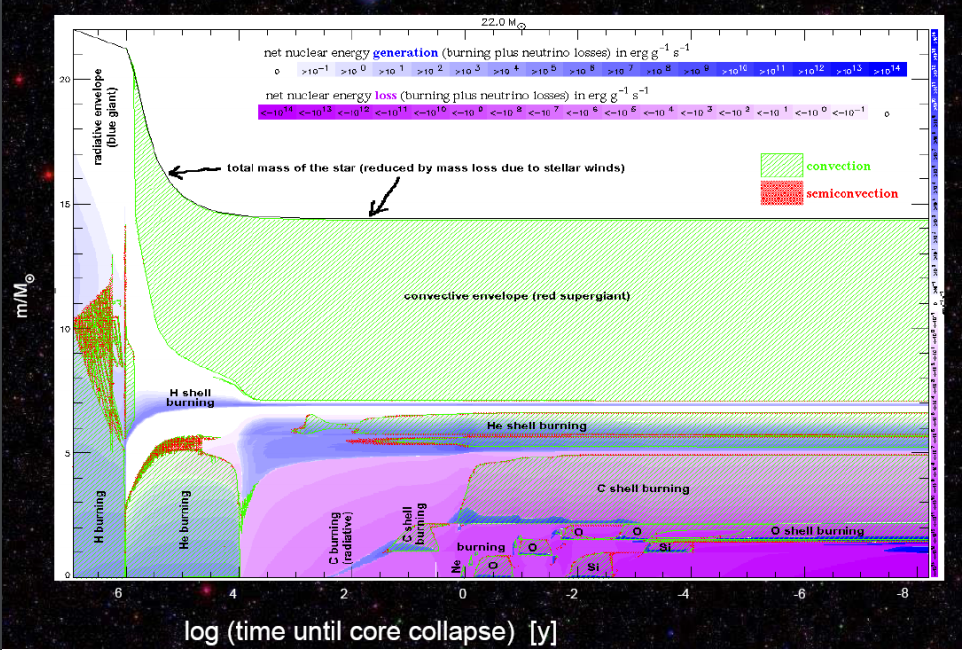
\includegraphics[width=12cm]{images/KippenhahnDiagram.png}
            \end{center}
            Jak widać poprzez wiatr gwiazda utraciła ponad 30\% swojej masy, głównie na etapie spalania helu. Wraz z upływem czasu gwiazda przechodzi na syntezę coraz to cięższych pierwiastków. Jednocześnie procesy z poprzednich etapów nadal są syntezowane poza jadrem – w powłokach otaczających jądro. Gdy gwiazda zaczyna odkładać już żelazo, to jej wnętrze wykazuje strukturę jak ogr (cebula). Im bliżej centrum tym cięższe pierwiastki są syntezowane, a całość zanurzona jest w chłodnej otoczce wodorowej – gwiazda jest \textbf{czerwonym nadolbrzymem}.
            \begin{center}
                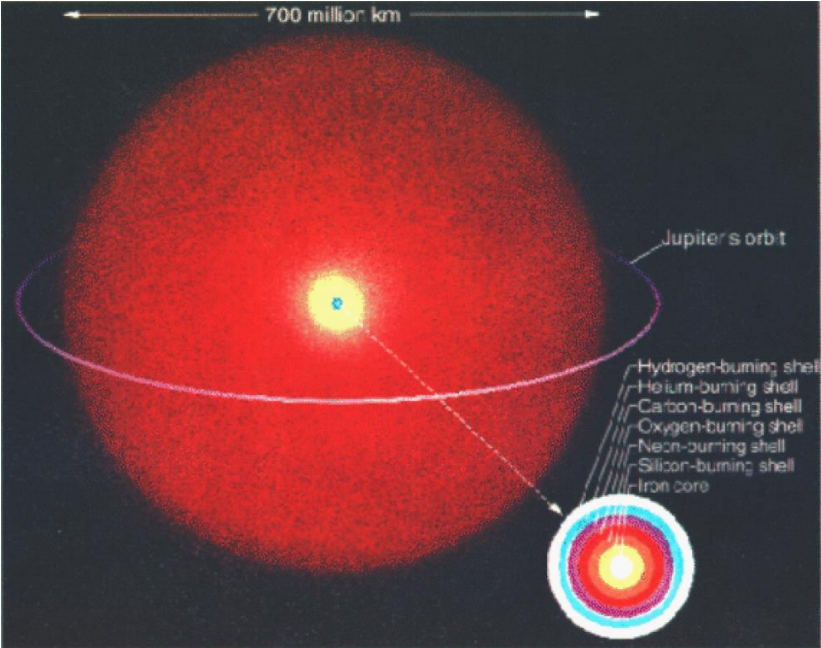
\includegraphics[width=12cm]{images/ogreStar.png}
            \end{center}
            \textbf{Gwiazdy Wolfa-Rayeta} – najbardziej typowi przedstawiciele wyewoluowanych, bardzo masywnych gwiazd. Zwykle w ich widmie trudno wykryć wodór, ponieważ jego większość została już przekształcona w cięższe pierwiastki lub zdmuchnięta wiatrem gwiazdowym. Przykładowa ścieżka rozwoju gwiazdy masywnej (\(15 \leq M_\odot \leq 25M_\odot\)): ciąg główny \(\to \) niebieski nadolbrzym \( \to \) czerwony nadolbrzym \(\to \) \textbf{supernowa} typu drugiego. Drugi przykład (\(25 M\odot \leq  M \leq 50 M_\odot\))(WNL, WNE i WC to gwiazdy Wolfa-Rayeta): ciąg główny \(\to \) niebieski nadolbrzym \( \to \) czerwony nadolbrzym \(\to \) WNL \(\to \) WNE \(\to \) WC \(\to \) supernowa typu Ib.
        \subsection{Śmierć gwiazd masywnych – supernowa}
            W jądrze żelazowym nie mogą już zachodzi procesy syntezy. Dodatkowo zaczynają pojawia się reakcje, w wyniku których neutrina unoszą sporo ilości energii tym samym destabilizując równowagę hydrostatyczną (i degenerując materię w jądrze) (fotodezintegracja jądra i wychwyt elektronu):
            \begin{align}
                ^{56}F + \gamma \to& 13 \:^4He + 4n - 2 MeV \\
                ^4He  + \gamma \to& 2p + 2n - 7MeV \\
                p^{ +} + e^{ -} \to& n + v_e
            \end{align}
            W pewnym momencie dochodzi do \textbf{kolapsu grawitacyjnego} – spadku swobodnego materii jądra z prędkością \(0.25 c\). Kolaps ulega zatrzymaniu przez ciśnienie zdegenerowanych neutronów (bo to fermiony – zakaz Pauliego), gdy jądro ma rozmiary \(10 - 100km\) i \(T\sim 2 \cdot 10^{10}K\), \(\rho \sim 10^{15} \frac{g}{cm^3}\). Powstaje zaczątek \textbf{gwiazdy neutronowej} Większość energii wydzielonej w wyniku kolapsu unoszona jest przez neutrina. Dla gęstości większej niż \(10^{12}\frac{g}{cm^3}\) materia staje się nieprzezroczysta dla neutrin i za odprowadzanie energii odpowiada konwekcja. Formująca się gwiazda neutronowa relaksuje się do większej objętości (\textbf{odbicie jądra}), ekspansje zatrzymuje napływ materii z otoczki: w pewnej odległości od centrum gwiazdy formuje się fala stojąca – miejsce dynamicznej równowagi między eksplozją i implozją.\\
            Decydującą dla kierunku dalszej propagacji fali stojącej jest efektywność konwekcji w rejonie centrum gwiazdy:
            \begin{itemize}
                \item jeśli umożliwia ona neutrinom zasilanie ekspansji, otoczka ulegnie odrzuceniu i formuje się gwiazda neutronowa.
                \item jeśli energia pozostaje zamknięta w centralnej części gwiazdy, napływająca materia powoduje wzrost masy jadra neutronowego powyżej trzech mas Słońca. Ciśnienie neutronów przestaje powstrzymywać kolaps grawitacyjny i formuje się \textbf{czarna dziura}.
            \end{itemize}
            Całemu procesowi kolapsu towarzyszy bardzo jasny rozbłysk – \textbf{supernowa}. Jej jasność porównywalna jest z jasnością całych galaktyk, mimo tego, że tylko 1\% energii wydzielonej w tym procesie unoszone jest przez fotony (90\% neutrina i 9\% wyrzucenie zewnętrznych części gwiazdy). Wyróżnia się typy supernowych: Ia, Ib, Ic i II. Jedynie Ia nie jest związany z kolapsem gwiazdy masywnej. Typy Ib i Ic wiąże się z gwiazdami Wolfa-Rayeta, a typ II z czerwonymi nadolbrzymami.\\
            Podsumowując ewolucje gwiazd:
            \begin{itemize}
                \item Gwiazdy najbardziej masywne syntezują w swych jądrach pierwiastki aż po żelazo i kończą ewolucję wybuchem supernowej, zamieniając się w gwiazdę neutronową albo w czarna dziurę.
                \item Gwiazdy o pośrednich masach syntezują w s

            \end{itemize}
\end{document}